% Figure 1
\ffigbox[\FBwidth]{%
\label{Fig:td2ex9}
}{
    \fbox{
        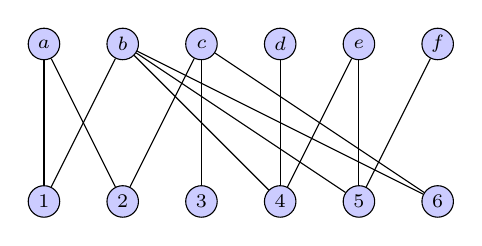
\begin{tikzpicture}[scale=1, every node/.style={circle, draw, fill=blue!20, inner sep=1pt, font=\scriptsize, minimum size=4mm}]
            \node (a) at (0, 2) {\(a\)};
            \node (b) at (1, 2) {\(b\)};
            \node (c) at (2, 2) {\(c\)};
            \node (d) at (3, 2) {\(d\)};
            \node (e) at (4, 2) {\(e\)};
            \node (f) at (5, 2) {\(f\)};

            \node (1) at (0, 0) {\(1\)};
            \node (2) at (1, 0) {\(2\)};
            \node (3) at (2, 0) {\(3\)};
            \node (4) at (3, 0) {\(4\)};
            \node (5) at (4, 0) {\(5\)};
            \node (6) at (5, 0) {\(6\)};

            \draw (a) -- (1);
            \draw (a) -- (2);

            \draw (b) -- (1);
            \draw (b) -- (4);
            \draw (b) -- (5);
            \draw (b) -- (6);
            
            \draw (c) -- (2);
            \draw (c) -- (3);
            \draw (c) -- (6);
            
            \draw (d) -- (4);
            
            \draw (e) -- (4);
            \draw (e) -- (5);
            
            \draw (f) -- (5);
        \end{tikzpicture}
    }
}